% Template for Cogsci submission with R Markdown

% Stuff changed from original Markdown PLOS Template
\documentclass[10pt, letterpaper]{article}

\usepackage{cogsci}
\usepackage{pslatex}
\usepackage{float}
\usepackage{caption}

% amsmath package, useful for mathematical formulas
\usepackage{amsmath}

% amssymb package, useful for mathematical symbols
\usepackage{amssymb}

% hyperref package, useful for hyperlinks
\usepackage{hyperref}

% graphicx package, useful for including eps and pdf graphics
% include graphics with the command \includegraphics
\usepackage{graphicx}

% Sweave(-like)
\usepackage{fancyvrb}
\DefineVerbatimEnvironment{Sinput}{Verbatim}{fontshape=sl}
\DefineVerbatimEnvironment{Soutput}{Verbatim}{}
\DefineVerbatimEnvironment{Scode}{Verbatim}{fontshape=sl}
\newenvironment{Schunk}{}{}
\DefineVerbatimEnvironment{Code}{Verbatim}{}
\DefineVerbatimEnvironment{CodeInput}{Verbatim}{fontshape=sl}
\DefineVerbatimEnvironment{CodeOutput}{Verbatim}{}
\newenvironment{CodeChunk}{}{}

% cite package, to clean up citations in the main text. Do not remove.
\usepackage{apacite}

% KM added 1/4/18 to allow control of blind submission


\usepackage{color}

% Use doublespacing - comment out for single spacing
%\usepackage{setspace}
%\doublespacing


% % Text layout
% \topmargin 0.0cm
% \oddsidemargin 0.5cm
% \evensidemargin 0.5cm
% \textwidth 16cm
% \textheight 21cm

\title{Children's shift from CDS to ADS vocabulary across early
childhood}

\usepackage{booktabs}
\usepackage{longtable}
\usepackage{array}
\usepackage{multirow}
\usepackage{wrapfig}
\usepackage{float}
\usepackage{colortbl}
\usepackage{pdflscape}
\usepackage{tabu}
\usepackage{threeparttable}
\usepackage{threeparttablex}
\usepackage[normalem]{ulem}
\usepackage{makecell}
\usepackage{xcolor}

\author{{\large \bf Kennedy Casey (kbcasey@uchicago.edu)}  \\{\large \bf Marisa Casillas (mcasillas@uchicago.edu)} \\Comparative Human Development, University of Chicago \\ Chicago, IL 60637 USA}

\newlength{\cslhangindent}
\setlength{\cslhangindent}{1.5em}
\newenvironment{CSLReferences}%
  {}%
  {\par}

\begin{document}

\maketitle

\begin{abstract}
abstract text here. abstract text here. abstract text here. abstract
text here. abstract text here. abstract text here. abstract text here.
abstract text here. abstract text here. abstract text here. abstract
text here. abstract text here. abstract text here. abstract text here.
abstract text here. abstract text here. abstract text here. abstract
text here. abstract text here. abstract text here. abstract text here.
abstract text here. abstract text here. abstract text here. abstract
text here. abstract text here. abstract text here. abstract text here.
abstract text here. abstract text here. abstract text here. abstract
text here. abstract text here. abstract text here. abstract text here.
abstract text here. abstract text here. abstract text here. abstract
text here. abstract text here. abstract text here. abstract text here.
abstract text here. abstract text here. abstract text here. abstract
text here. abstract text here. abstract text here.

\textbf{Keywords:}
child-directed speech; word production; linguistic input; social
register; corpus analysis; developmental change
\end{abstract}

\hypertarget{introduction}{%
\section{Introduction}\label{introduction}}

\hypertarget{methods}{%
\section{Methods}\label{methods}}

\hypertarget{corpus-and-item-selection}{%
\subsection{Corpus and item selection}\label{corpus-and-item-selection}}

We analyzed 8251 transcripts in the North American English collection of
the Child Language Data Exchange System (CHILDES) database (MacWhinney,
2000). The included transcripts were drawn from 52 individual corpora
and featured 980 children up to 7 years of age (range = 1--84 months,
\emph{M} = 33.5 months).

15 CDS/ADS word pairs were selected as test items based on their
appearance on the MacArthur-Bates Communicative Development Inventory
(Fenson et al., 1994) and their frequency of occurrence in CHILDES (at
least 100 child-produced tokens and 100 other-produced tokens; see Table
\ref{tab:tab1}).

Cases where the same object, animal, or routine could be reasonably
labeled with either form in typical communicative interactions with
young children.

\begin{table}[ht]
\centering
\fontsize{6}{8}\selectfont
\begin{tabular}{r>{}lrrrr}
  \toprule
\multicolumn{2}{c}{\textbf{ }} & \multicolumn{2}{c}{\textbf{CDS tokens by speaker}} & \multicolumn{2}{c}{\textbf{ADS tokens by speaker}} \\
\cmidrule(l{3pt}r{3pt}){3-4} \cmidrule(l{3pt}r{3pt}){5-6}
\textbf{} & \textbf{Pair} & \textbf{Child} & \textbf{Other} & \textbf{Child} & \textbf{Other }\\ 
  \midrule
1 & \em{doggy/dog} & 2249 & 2644 & 3519 & 5113 \\ 
  2 & \em{kitty/cat} & 1552 & 3309 & 2779 & 4443 \\ 
  3 & \em{tummy/stomach} & 435 & 623 & 112 & 360 \\ 
  4 & \em{daddy/dad} & 9603 & 10048 & 2313 & 1031 \\ 
  5 & \em{mommy/mom} & 20294 & 17070 & 7616 & 2552 \\ 
  6 & \em{bunny/rabbit} & 1237 & 2597 & 1060 & 1397 \\ 
  7 & \em{duckie/duck} & 307 & 647 & 1933 & 3003 \\ 
  8 & \em{blankie/blanket} & 174 & 224 & 825 & 874 \\ 
  9 & \em{froggy/frog} & 154 & 434 & 970 & 1846 \\ 
  10 & \em{potty/bathroom} & 511 & 786 & 161 & 270 \\ 
  11 & \em{night night/goodnight} & 149 & 153 & 102 & 446 \\ 
  12 & \em{dolly/doll} & 745 & 1054 & 674 & 2697 \\ 
  13 & \em{horsey/horse} & 1149 & 1034 & 1749 & 2575 \\ 
  14 & \em{piggy/pig} & 405 & 1212 & 1276 & 2139 \\ 
  15 & \em{birdie/bird} & 399 & 588 & 1879 & 3358 \\ 
   \bottomrule
\end{tabular}
\caption{CHILDES frequency for 15 CDS/ADS word pairs. Child-produced counts 
                             include tokens produced only by the target child. All other 
                             speakers' productions are included in the other-produced counts.} 
\label{tab:tab1}
\end{table}

\hypertarget{linguistic-predictors}{%
\subsection{Linguistic predictors}\label{linguistic-predictors}}

All analyses were conducted over individual utterances. We quantified
prosodic, lexical and syntactic information to describe each utterance
containing one of the 30 target words.

\hypertarget{prosodic-level}{%
\subsubsection{Prosodic level}\label{prosodic-level}}

For all timestamped utterances (41.4\% of child-produced and 42.3\% of
other-produced utterances), mean pitch and pitch range were extracted
using Praat software (Boersma \& Weenink, 2016). Speech rate was
calculated as the number of words produced per second. Utterances
shorter than 58 ms were excluded from analysis. This lower bound was set
by identifying the the shortest possible duration of an utterance
containing at least one word in four manually annotated North American
English corpora in HomeBank (Bergelson, 2016; McDivitt \& Soderstrom,
2016; VanDam et al., 2016; VanDam, 2016; Warlaumont \& Pretzer, 2016;
see also Bergelson et al., 2019).

\hypertarget{lexical-level}{%
\subsubsection{Lexical level}\label{lexical-level}}

Typically, measures of lexical complexity are calculated over at least
minutes or hours of transcribed speech rather than individual
utterances. Here, we aimed to estimate local lexical complexity in two
ways.

First, we calculated the negative log proportion of known words in each
utterance (consistent with Foushee, Griffiths, \& Srinivasan, 2016;
Kidd, Piantadosi, \& Aslin, 2012). A word was considered `known' if the
age of acquisition estimate (AoA) Frank, Braginsky, Yurovsky, \&
Marchman (2017) was less than or equal to the age of the target child
when they heard or produced the utterance. Utterances with
proportionally fewer known words are \emph{more} lexically complex.

To account for more individual variation in word production, we included
a measure

\hypertarget{syntactic-level}{%
\subsubsection{Syntactic level}\label{syntactic-level}}

Syntactic measures included both the number of verb phrases and length
(in words) of each utterance. Words were chosen over morphemes in the
length analysis because we identified systematic errors in automatic
morpheme counts. Manual checking of 5\% of target utterances (i.e., XXXX
utterances) revealed an error rate of XX\%.

\hypertarget{results}{%
\section{Results}\label{results}}

\hypertarget{measuring-production-when-do-children-produce-cds-vs.-ads-forms}{%
\subsection{Measuring production: When do children produce CDS vs.~ADS
forms?}\label{measuring-production-when-do-children-produce-cds-vs.-ads-forms}}

\hypertarget{characterizing-the-input-in-what-linguistic-contexts-do-children-hear-cds-vs.-ads-forms}{%
\subsection{Characterizing the input: In what linguistic contexts do
children hear CDS vs.~ADS
forms?}\label{characterizing-the-input-in-what-linguistic-contexts-do-children-hear-cds-vs.-ads-forms}}

We used mixed-effects binomial logistic regression models to predict the
appearance of CDS vs.~ADS forms in given utterance on the basis of
target child's age, several linguistic properties of the utterance, and
interactions between each property and age. Models included random
intercepts for individual word pairs and speakers and were fitted to all
utterance data from speakers other than the target child.

\begin{CodeChunk}
\begin{figure}[H]

{\centering 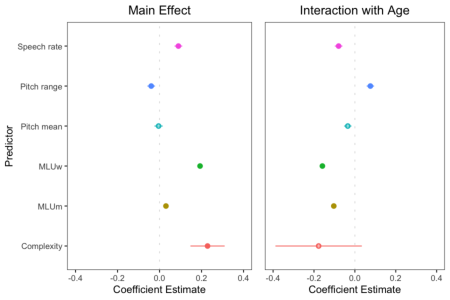
\includegraphics{figs/model-plot-1} 

}

\caption[Coefficient estimates for linguistic predictors of form]{Coefficient estimates for linguistic predictors of form. Positive main effects indicate that utterances with higher levels of the predictor are more likely to contain ADS forms, relative to CDS forms. Positive age interactions indicate an increasing effect of the predictor with age. Error bars depict standard errors of the coefficient estimates, and filled circles represent significant effects (\textit{p} $<$ 0.05).}\label{fig:model-plot}
\end{figure}
\end{CodeChunk}

\hypertarget{modeling-learning-what-linguistic-information-can-be-used-to-distinguish-cds-vs.-ads-contexts}{%
\subsection{Modeling learning: What linguistic information can be used
to distinguish CDS vs.~ADS
contexts?}\label{modeling-learning-what-linguistic-information-can-be-used-to-distinguish-cds-vs.-ads-contexts}}

\hypertarget{discussion}{%
\section{Discussion}\label{discussion}}

\hypertarget{acknowledgements}{%
\section{Acknowledgements}\label{acknowledgements}}

We are grateful to Claire Bergey, Ruthe Foushee, Ben Morris, and the
members of the University of Chicago Chatter Lab and Northwestern
University Child Language Lab for valuable discussion and feedback on
this work.

\hypertarget{references}{%
\section{References}\label{references}}

\setlength{\parindent}{-0.1in} 
\setlength{\leftskip}{0.125in}

\noindent

\hypertarget{refs}{}
\begin{CSLReferences}{1}{0}
\leavevmode\hypertarget{ref-bergelsoncorpus}{}%
Bergelson, E. (2016). Bergelson HomeBank corpus.
\url{https://doi.org/10.21415/T5PK6D}.

\leavevmode\hypertarget{ref-bergelson2019north}{}%
Bergelson, E., Casillas, M., Soderstrom, M., Seidl, A., Warlaumont, A.
S., \& Amatuni, A. (2019). What do north american babies hear? A
large-scale cross-corpus analysis. \emph{Developmental Science},
\emph{22}(1), e12724.

\leavevmode\hypertarget{ref-boersma2016praat}{}%
Boersma, P., \& Weenink, D. (2016). Praat software. \emph{Amsterdam:
University of Amsterdam}.

\leavevmode\hypertarget{ref-fenson1994variability}{}%
Fenson, L., Dale, P. S., Reznick, J. S., Bates, E., Thal, D. J.,
Pethick, S. J., \ldots{} Stiles, J. (1994). Variability in early
communicative development. \emph{Monographs of the Society for Research
in Child Development}, i--185.

\leavevmode\hypertarget{ref-foushee2016lexical}{}%
Foushee, R., Griffiths, T., \& Srinivasan, M. (2016). Lexical complexity
of child-directed and overheard speech: Implications for learning. In
\emph{Proceedings of the 38th annual conference of the cognitive science
society} (pp. 1697--1702).

\leavevmode\hypertarget{ref-frank2017wordbank}{}%
Frank, M. C., Braginsky, M., Yurovsky, D., \& Marchman, V. A. (2017).
Wordbank: An open repository for developmental vocabulary data.
\emph{Journal of Child Language}, \emph{44}(3), 677--694.

\leavevmode\hypertarget{ref-kidd2012goldilocks}{}%
Kidd, C., Piantadosi, S. T., \& Aslin, R. N. (2012). The goldilocks
effect: Human infants allocate attention to visual sequences that are
neither too simple nor too complex. \emph{PloS One}, \emph{7}(5),
e36399.

\leavevmode\hypertarget{ref-macwhinney2000childes}{}%
MacWhinney, B. (2000). \emph{The CHILDES project: The database} (Vol.
2). Psychology Press.

\leavevmode\hypertarget{ref-soderstromcorpus}{}%
McDivitt, K., \& Soderstrom, M. (2016). McDivitt HomeBank corpus.
\url{https://doi.org/10.21415/T5KK6G}.

\leavevmode\hypertarget{ref-vandamcorpus}{}%
VanDam, M. (2016). VanDam2 HomeBank corpus.

\leavevmode\hypertarget{ref-homebank}{}%
VanDam, M., Warlaumont, A. S., Bergelson, E., Cristia, A., De Palma, P.,
\& MacWhinney, B. (2016). Homebank: An online repository of daylong
child-centered audio recordings. \url{https://homebank.talkbank.org}.

\leavevmode\hypertarget{ref-warlaumontcorpus}{}%
Warlaumont, A. S., \& Pretzer, G. M. (2016). Warlaumont HomeBank corpus.
\url{https://doi.org/10.21415/t54s3c}.

\end{CSLReferences}

\bibliographystyle{apacite}


\end{document}
